% =====================================================================
% LADC 2026 Student Forum paper — ENGLISH version
% Format: Springer LNCS (llncs.cls)
% Scope: empirical dependability measurement (NO SPN modeling)
%
% BUILD: requires llncs.cls
%   pdflatex artigo_en.tex  (twice for references)
% =====================================================================
\documentclass[runningheads]{llncs}

\usepackage[T1]{fontenc}
\usepackage[utf8]{inputenc}
\usepackage{graphicx}
\usepackage{booktabs}
\usepackage{amsmath}
\usepackage{url}
\usepackage{float}
\usepackage[table]{xcolor}
% DOI quebrável em fonte romana (o \doi do llncs é inquebrável e estica linhas)
\AtBeginDocument{\def\doi#1{{\urlstyle{rm}\url{https://doi.org/#1}}}}
\def\UrlBreaks{\do\/\do\-\do\.\do\_}
% --- spacing adjustments for the LADC 11-page limit ---
\usepackage{enumitem}
\setlist{nosep,topsep=2pt,leftmargin=*}
\setlength{\textfloatsep}{10pt plus 2pt minus 2pt}
\setlength{\floatsep}{8pt plus 2pt minus 2pt}
\setlength{\intextsep}{10pt plus 2pt minus 2pt}
\setlength{\abovecaptionskip}{6pt}
\setlength{\belowcaptionskip}{0pt}

\begin{document}

\title{Empirical Dependability Measurement of Apache Cassandra under
Fault Injection: the Impact of Consistency Levels}
\titlerunning{Cassandra Dependability under Fault Injection}

% If the forum is double-blind, comment out the authors for submission.
\author{Caio Farias Cavalcanti\inst{1} \and
Gustavo Rau de Almeida Callou\inst{1}}
\authorrunning{C. F. Cavalcanti and G. R. A. Callou}
\institute{Federal Rural University of Pernambuco (UFRPE), Recife--PE, Brazil\\
\email{\{caio.farias,gustavo.callou\}@ufrpe.br}}

\maketitle

\begin{abstract}
Distributed database systems such as Apache Cassandra offer tunable consistency
levels that regulate the trade-off between availability and consistency. Well
understood in theory, this trade-off nonetheless lacks empirical measurements of
how different consistency levels affect service dependability under real faults.
This work presents a measurement study that injects five fault types (replica
crash, coordinator crash, network delay, packet loss, and network partition)
into Cassandra under three consistency levels (ONE, QUORUM, ALL) and three load
levels, with three repetitions each (135 runs). The results quantify two
distinct phenomena: faults that cause unavailability (crash and partition), where
ONE and QUORUM completely mask the fault while ALL exhibits an error rate of up
to 25\%; and timing faults (delay and loss), where throughput degrades by
$\sim$98\% regardless of the consistency level. We further measure the time to
repair (MTTR) per fault type, from $\sim$15\,s (crash) to $\sim$32\,s
(partition). The measurements extend prior work by introducing partition
scenarios not previously studied and by providing empirical observed service
availability and MTTR values.

\keywords{Dependability \and Apache Cassandra \and Fault injection \and
Consistency levels \and Availability \and Fault tolerance.}
\end{abstract}

% =====================================================================
\section{Introduction}
% =====================================================================

Distributed NoSQL databases have become core infrastructure for large-scale
applications, offering horizontal scalability and fault tolerance through
replication. Apache Cassandra is a prominent representative of this category,
adopted by organizations requiring high availability over large data
volumes~\cite{lakshman2010cassandra}. A defining feature of Cassandra is
\emph{tunable consistency}: for each operation, the application chooses how many
replicas must participate, explicitly regulating the consistency--availability
trade-off predicted by the CAP theorem~\cite{brewer2000cap,gilbert2002cap}.

This trade-off is well understood at a theoretical level. What remains less
explored is the \emph{empirical quantification} of how the choice of consistency
level affects the dependability of the service delivered to the client when the
system faces real faults. Knowing that ALL ``prioritizes consistency'' does not
tell \emph{how much} availability is lost under a concrete fault, nor \emph{how
quickly} the service recovers. These are dependability measures~\cite{avizienis2004basic,meyer1980}
that operators need to make informed configuration decisions.

The object of study is the consistency level, and Cassandra suits it because the
level is chosen per operation: ONE, QUORUM and ALL can be compared on the
\emph{same} cluster, data and fault. In consensus-based systems such as etcd
(Raft), the guarantee is largely fixed by the protocol. The injection method
(\texttt{systemctl}, \texttt{tc/netem}, \texttt{iptables}, client-side time
series) does not depend on Cassandra; whether the trade-offs generalize is left
to future work.

This work addresses that gap through a controlled measurement study: a
five-node Cassandra cluster in the cloud is subjected to five fault classes under
three consistency levels and three loads, and the throughput, latency and error
rate are recorded before, during and after each fault.

The contributions are: (i) a reproducible fault-injection methodology for
Cassandra, covering crash, timing, omission and partition faults with precise
timeline control, whose scripts and data are publicly
available~\cite{artifact}; (ii) the empirical quantification of the impact of the
consistency level on dependability, distinguishing availability faults from
timing faults; and (iii) measured availability and MTTR values, including
partition scenarios not addressed in related work. The scope is restricted to
measurement: this is the experimental stage of an undergraduate project, with
analytical modeling as the subsequent stage.

The study is guided by three research questions:
\begin{itemize}
\item \textbf{RQ1:} How does the Cassandra consistency level affect service
availability under crash and network partition faults?
\item \textbf{RQ2:} How does the consistency level affect performance
degradation under network timing faults (delay and packet loss)?
\item \textbf{RQ3:} How do different fault types affect Cassandra recovery time
(MTTR)?
\end{itemize}

Section~\ref{sec:related} reviews related work and Section~\ref{sec:background}
the concepts used. Section~\ref{sec:methodology} describes the experimental
design and Section~\ref{sec:environment} the apparatus.
Section~\ref{sec:casestudy} presents and discusses the results, and
Section~\ref{sec:conclusion} concludes.

% =====================================================================
\section{Related Work}
\label{sec:related}
% =====================================================================

Dependability evaluation of Cassandra has been approached through measurement
and through analytical modeling. Ferreira et al.~\cite{ferreira2021}
experimentally evaluated Cassandra's performance under different consistency
levels and loads, establishing a baseline of throughput and latency under normal
operation. That work, however, focuses on the fault-free regime and does not
characterize system behavior under node unavailability or network degradation.
The present study adopts compatible load parameters for comparability, but
extends the evaluation with a systematic fault-injection phase.

Other empirical studies cover complementary dimensions. Rosselli et
al.~\cite{rosselli2016} evaluated Cassandra's availability and fault tolerance by
measuring the impact of a node failure on throughput and latency, without
systematically varying the consistency level or covering network faults such as
delay, loss and partition. Rahman et al.~\cite{rahman2012} proposed a framework,
integrated with YCSB, for empirically measuring consistency anomalies in
key-value stores, a perspective orthogonal to this work, which centers on
availability and recovery. In failure-oriented testing, the Jepsen
project~\cite{jepsen} became a reference by subjecting distributed databases,
including Cassandra, to partitions and crashes in order to verify
\emph{correctness violations} of consistency guarantees; our work differs in goal
and method, quantifying dependability metrics (error rate, throughput degradation
and MTTR) as a function of the consistency level, under a controlled fault
timeline.

Gomes et al.~\cite{gomes2019} proposed an analytical dependability model for
Cassandra based on generalized stochastic Petri nets (GSPN), estimating
availability from MTTF and MTTR parameters adopted hypothetically (MTTF of
2880\,h and 5760\,h; MTTR of 0.5\,h and 1\,h), in the absence of direct
measurements. Since the quality of an analytical model depends on its input
parameters, this work contributes \emph{empirically measured} MTTR values per
fault type.

Fault injection is a well-established \emph{fault forecasting} technique for the
experimental evaluation of
dependability~\cite{avizienis2004basic,borges2025,silva2025models}. Network
partitions, which materialize the CAP trade-off, have not, to our knowledge, been
characterized as a dependability measure in the related Cassandra studies.

% =====================================================================
\section{Background}
\label{sec:background}
% =====================================================================

\subsection{Dependability and the fault--error--failure chain}

Dependability is the ability of a system to deliver a service that can
justifiably be trusted~\cite{avizienis2004basic}, encompassing attributes such as
availability (readiness for correct service), reliability (continuity of correct
service) and maintainability (ability to undergo repair). The Avi\v{z}ienis et
al. framework structures dependability threats along the causal chain \emph{fault
$\rightarrow$ error $\rightarrow$ failure}: a \textbf{fault} is the hypothesized
or actual cause of an error (e.g., a process terminating); an \textbf{error} is
the part of the system state that may lead to a failure (e.g., an unreachable replica);
and a \textbf{failure} occurs when the delivered service deviates from the correct
one (e.g., an operation returning an error to the client). Between error and failure act the \emph{fault
tolerance mechanisms}: when a mechanism prevents an error from propagating to the
service, the fault is said to be \emph{masked}; controlled fault injection
measures whether each fault crosses these defenses.

\subsection{Cassandra's replication and consistency levels}

Cassandra partitions data over a \emph{token} ring and replicates each partition
across a number of nodes given by the \emph{replication factor} ($RF$). With $RF=3$, each data item exists on three distinct nodes,
which constitutes its fundamental fault tolerance mechanism.

The \emph{consistency level} (CL) determines, per operation, how many replicas
must respond for it to be considered successful: \textbf{ONE} requires a single
replica (tolerates the loss of up to $RF-1$ replicas);
\textbf{QUORUM} requires a majority, $\lfloor RF/2 \rfloor + 1$ replicas (two,
for $RF=3$; tolerates the loss of one); and \textbf{ALL} requires all $RF$
replicas (tolerates no loss).

A consistency level is a per-operation parameter, not a consistency
\emph{model}; the model it yields depends on the levels used for reads ($R$
replicas) and writes ($W$). With ONE, a read may return stale data, and the
system offers only \emph{eventual consistency}. When $R+W>RF$, as with QUORUM
for both or ALL, every read set intersects the replicas that acknowledged the
latest completed write. This is still weaker than \emph{linearizability}, which
in Cassandra requires \emph{lightweight transactions} (Paxos), not used here. We
measure the availability and performance \emph{cost} of each level, not the
consistency obtained, which is the subject of~\cite{rahman2012,jepsen}.

The CL is thus an application-level mechanism for controlling the behavior
observed during node and network failures: ONE favors availability (responding
with any reachable replica), while ALL refuses to respond without all of them. An important aspect for interpreting the results is that,
in Cassandra, \emph{every write is sent to all replicas} regardless of the CL,
which defines only how many acknowledgments the coordinator waits for.

\subsection{Measurable dependability attributes}

From observing the service under faults we derive the measures of interest,
drawing on two complementary traditions: the attributes of the taxonomy of
Avi\v{z}ienis et al.~\cite{avizienis2004basic} and Meyer's
\emph{performability}~\cite{meyer1980}. \textbf{Availability} (readiness for
correct service) is measured at the operational level, by the fraction of
operations served correctly, $A = 1 - (\text{errors}/\text{total operations})$;
we call this \emph{observed service availability}. It departs from the classical
steady-state availability $A = \text{MTTF}/(\text{MTTF}+\text{MTTR})$ for two
reasons: faults are injected at fixed instants, so there is no MTTF to measure;
and in a request-serving system each operation is a demand for service, so the
fraction served correctly is the availability the client experiences, the
request-based form used in service-level objectives. Since it depends on the
observation interval, we report it over the whole run and inside the fault
window.
\textbf{Performability}~\cite{meyer1980} is the degree of throughput and latency
degradation during the fault, when the service remains available but with reduced
quality; it is not an attribute of the Avi\v{z}ienis et al. taxonomy, but a
composite measure of performance and dependability suited to degradable systems.
\textbf{Maintainability} is assessed through the recovery time (MTTR) after the
injected fault.

% =====================================================================
\section{Methodology}
\label{sec:methodology}
% =====================================================================

\subsection{Experimental design}

The study is organized in two phases. The \emph{baseline phase} measures
throughput and latency under normal operation, varying the consistency level
(ONE, QUORUM, ALL) and the load (10, 30 and 50 client threads), with three
repetitions per cell. The \emph{fault-injection phase} adds the fault-type
dimension, totaling $5 \times 3 \times 3 \times 3 = 135$ controlled runs.

\subsection{Injected fault types}

Five fault types cover the main classes of the dependability taxonomy.
\textbf{Replica crash} (\texttt{node\_crash}): termination of the Cassandra process
on a replica node, via \texttt{systemctl stop}, which tests masking by
replication. This is an \emph{orderly} shutdown, in which the node announces its
departure to its peers; we chose it to isolate replica loss from
failure-detection delay and to restart cleanly in a long automated battery
(abrupt termination is discussed in the threats to validity). \textbf{Coordinator crash} (\texttt{coord\_crash}): termination of the
process on the client's contact node, testing the \emph{driver}'s routing
failover.
\textbf{Network delay} (\texttt{net\_delay}): insertion of
$200\,\text{ms} \pm 50\,\text{ms}$ of latency into a node's egress traffic, via
\texttt{tc/netem} (a timing fault). \textbf{Packet loss} (\texttt{net\_loss}):
dropping 25\% of a node's egress packets, also via \texttt{tc/netem} (an
omission fault). \textbf{Network partition} (\texttt{net\_partition}): isolation of
one node from the others, via \texttt{iptables} rules, keeping the node alive but
unable to communicate; it materializes the CAP theorem scenario.

\subsection{Per-run timeline}

Each run lasts 300\,s and follows a controlled timeline
(Fig.~\ref{fig:timeline}): 60\,s healthy; fault injection at $t=60\,$s; the fault
held for 90\,s; removal at $t=150\,$s; and recovery until $t=300\,$s. The 90\,s
window exceeds the fault detection time of Cassandra's \emph{gossip} protocol (on
the order of 10\,s), ensuring an effectively-detected fault window long enough for
measurement.

% ---- FIGURE 1: run timeline ----
\begin{figure}[t]
\centering
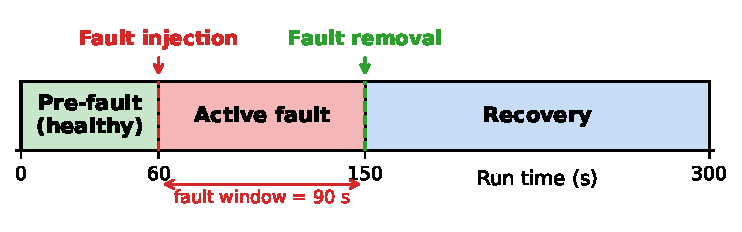
\includegraphics[width=0.75\textwidth]{figs/fig_timeline_en.pdf}
\caption{Controlled timeline of a fault-injection run.}
\label{fig:timeline}
\end{figure}

\subsection{Workload and metrics}

The load is generated by YCSB (Yahoo! Cloud Serving Benchmark)~\cite{ycsb} with
\emph{Workload~A} (50\% reads, 50\% updates) over 100,000 records. Each run is
bounded by wall-clock time (300\,s) rather than by operation count, ensuring the
fault window occurs within the measurement period. YCSB records every 10\,s the
throughput, latency and counts of successful and failed operations, constituting
the time series from which we derive the metrics; the actual injection, removal
and recovery instants are recorded by the injection harness, allowing the series
to be aligned to the pre-fault, during-fault and post-fault windows.

From these series we compute the \textbf{error rate} (errors over total
operations) and the \textbf{observed service availability} ($1-$ error rate),
used for crash and partition; the \textbf{throughput degradation}
($1 - \text{throughput}_{\text{during}}/\text{throughput}_{\text{pre}}$), used for
delay and loss; and the \textbf{MTTR}, the interval between fault removal and the
confirmation, via \texttt{nodetool status}, that the cluster returned to a
five-node-up state. By construction, the MTTR is only meaningful for faults that
bring the node down from \emph{gossip} (crash and partition); for timing faults
the relevant recovery is that of throughput, observable in the post-fault
window.

% =====================================================================
\section{Environment and Experimental Apparatus}
\label{sec:environment}
% =====================================================================

\subsection{Infrastructure}

The experiment ran on the Google Cloud Platform, in the
\texttt{us-central1-a} zone (Fig.~\ref{fig:arquitetura}). The Cassandra cluster
comprises five
\texttt{e2-standard-2} virtual machines (2 vCPUs, 8\,GB RAM each) running
Cassandra~4.1 on Ubuntu~22.04, and load is generated by a dedicated VM
(\texttt{e2-medium}, 2 vCPUs, 4\,GB) co-located in the same zone so that
client--cluster latency ($\sim$0.3\,ms on the internal network) is not a
confounding factor.

\begin{figure}[t]
\centering
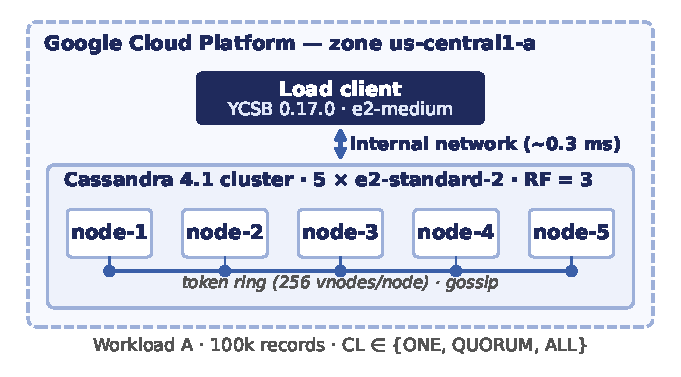
\includegraphics[width=0.72\textwidth]{figs/arch_en.pdf}
\caption{Architecture of the experimental environment: a Cassandra~4.1 cluster of
five \texttt{e2-standard-2} nodes (RF=3, \texttt{SimpleStrategy}) and the YCSB
load client (\texttt{e2-medium}), co-located in the \texttt{us-central1-a} zone of
the Google Cloud Platform.}
\label{fig:arquitetura}
\end{figure}

\subsection{Cassandra configuration}
\label{sec:cassandra-config}

The cluster uses $RF=3$ with \texttt{SimpleStrategy} replication (suitable for a
single datacenter), \texttt{num\_tokens}=256, \texttt{Murmur3\-Partitioner} and
the \texttt{Gossiping\-Property\-File\-Snitch}, with two \emph{seed} nodes. The
resulting
token distribution assigns each node $\sim$58--62\% of the key space in effective
ownership, which is relevant for interpreting the results under CL=ALL.

\subsection{Load and tooling}

Load generation uses YCSB~0.17.0~\cite{ycsb}. Fault injection is performed by
scripts that orchestrate, synchronized with the YCSB run, process termination and
restart (\texttt{systemctl}) for the crash scenarios, queueing discipline
manipulation (\texttt{tc/netem}) for delay and loss, and firewall rules
(\texttt{iptables}) for partition. Post-removal verification and idempotent
cleanup prevent residual fault state from contaminating subsequent runs, a
critical requirement in a long battery of automated runs. Table~\ref{tab:params}
summarizes the core experimental parameters. The fault-injection and analysis
scripts, the raw logs and the per-run data are publicly available~\cite{artifact}.

\begin{table}[t]
\centering
\scriptsize
\renewcommand{\arraystretch}{1.15}
\setlength{\tabcolsep}{3.5pt}
\caption{Experiment parameters.}
\label{tab:params}
\begin{tabular}{llll}
\toprule
\textbf{Parameter} & \textbf{Value} & \textbf{Parameter} & \textbf{Value} \\
\midrule
\rowcolor{gray!12}
Cassandra nodes & 5 $\times$ e2-standard-2 & Load (threads) & 10, 30, 50 \\
Load client & 1 $\times$ e2-medium & Repetitions per cell & 3 \\
\rowcolor{gray!12}
Cassandra version & 4.1 & Workload & YCSB A (50/50 read/update) \\
Replication factor & 3 (SimpleStrategy) & Records & 100,000 \\
\rowcolor{gray!12}
Consistency levels & ONE, QUORUM, ALL & Run duration & 300\,s \\
Total runs (faults) & 135 & Fault window & 90\,s ($t=60$--150\,s) \\
\bottomrule
\end{tabular}
\end{table}

% =====================================================================
\section{Case Study: Results and Discussion}
\label{sec:casestudy}
% =====================================================================

In the fault-free baseline, the coefficient of variation across repetitions
stayed below 3\%. The results are grouped by the predominant attribute:
availability (crash, partition) and performability (timing faults).

\subsection{Availability under crash and partition}

Table~\ref{tab:availability} presents the mean error rate per fault type and
consistency level. The pattern is clear and consistent with quorum theory: under
replica or coordinator crash, ONE and QUORUM maintain a near-zero error rate
(zero failed operations in every cell, except for a single one in
$2.6\times10^{7}$ under ONE for the coordinator crash), since with $RF=3$ the loss of
one replica leaves two available, sufficient for ONE (one) and QUORUM (two). The
fault is therefore \emph{masked} by replication, and both deliver $\sim$100\%
observed service availability. Under ALL, the requirement of all three replicas
causes every operation whose replica set includes the unavailable node to fail,
resulting in a mean error rate of $\sim$24--25\% over the entire run. This is lower than
the fraction of affected replicas because it is diluted by the healthy periods.

The dilution is not proportional to time (90 of 300\,s, 30\%). Throughput
after the fault ($\sim$4400--5700\,ops/s) is lower than before it
($\sim$7100--8200\,ops/s), so the fault window holds 33--41\% of the run's
operations. We attribute the lower post-fault throughput to the reintegration of
the node, which under ALL takes part in every operation on its replicas; this
explanation is inferred from Cassandra's behavior, not instrumented.

Measured \emph{inside the fault window}, from the 10\,s YCSB samples, the error
rate under ALL is 56.7\% for replica crash, 55.6\% for coordinator crash and
56.7\% for partition (standard deviation below 0.1 points). Replica crash and
partition target the \emph{same} node and agree to the third decimal (56.65\%
and 56.66\%): the fault type changes for how long operations fail, not which
ones. All three are close to the 60\% expected from $RF=3$ over five nodes under
uniform access; we attribute the gap to the \emph{zipfian} key distribution of
\emph{Workload~A}~\cite{ycsb}. Part of the errors occurs \emph{after} removal:
service returns $\sim$13--15\,s after a crash is removed and $\sim$3\,s after
the partition is removed. The mean rate (Table~\ref{tab:availability}) and the
instantaneous one are complementary: the former quantifies the amortized cost over
the entire run, the latter isolates the severity perceived while the node is in
fact unavailable.

\begin{table}[t]
\centering
\caption{Error rate (\%) per fault type and consistency level (mean $\pm$
standard deviation over loads and repetitions; $n=9$ per cell: 3 loads $\times$
3 repetitions). In parentheses, the absolute number of failed operations summed
over the nine runs; each cell totals $1.6$--$2.8\times10^{7}$ operations.}
\label{tab:availability}
\small
\setlength{\tabcolsep}{2.5pt}
\begin{tabular}{lccc}
\toprule
\textbf{Fault type} & \textbf{ONE} & \textbf{QUORUM} & \textbf{ALL} \\
\midrule
Replica crash      & 0.00$\pm$0.00 (0) & 0.00$\pm$0.00 (0) & 24.29$\pm$4.24 (3{,}902{,}961) \\
Coordinator crash  & 0.00$\pm$0.00 (1) & 0.00$\pm$0.00 (0) & 25.25$\pm$1.45 (4{,}008{,}616) \\
Network partition  & 0.05$\pm$0.05 (16{,}305) & 0.05$\pm$0.10 (9{,}768) & 19.01$\pm$1.74 (3{,}442{,}518) \\
\bottomrule
\end{tabular}
\end{table}

An original result lies in the comparison between crash and partition under ALL:
the partition produces a \emph{lower} mean error rate ($\sim$19\%) than the crash
($\sim$24--25\%), even though the instantaneous severity measured on the
\emph{same} target node is identical ($\sim$56.7\%). The difference does not lie in what
happens \emph{during} the fault, since under ALL an isolated but live node is as
unreachable as a dead one, but in the \emph{duration} of the service impairment: $\sim$98\,s under
partition against $\sim$124--129\,s under the crashes. Removing an \texttt{iptables} rule
restores connectivity at once, whereas a restarted process must first rejoin the
cluster. This dissociation between
\emph{fault removal} and \emph{service restoration} had not been characterized
in related work. Figure~\ref{fig:panel} (center) also shows a brief QUORUM error
spike ($\sim$18\%) in the first $\sim$10\,s of the partition, invisible in
aggregate metrics, which we attribute to \emph{gossip} convergence.

% ---- FIGURE 2: panel of the 3 key faults ----
\begin{figure}[t]
\centering
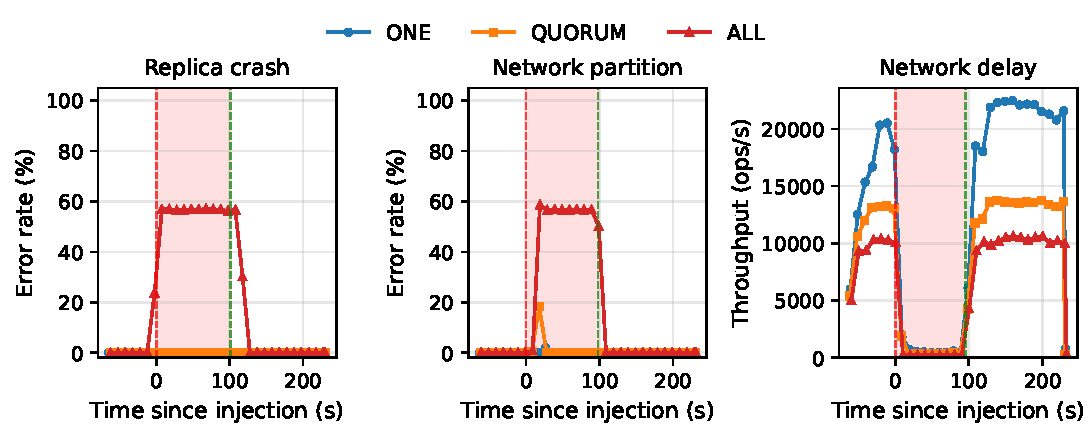
\includegraphics[width=\textwidth]{figs/panel_3faults_en.pdf}
\caption{Time series at 50 threads (median repetition), with time realigned to the
fault injection instant ($t=0$) and the fault window shaded. Left and center:
error rate under replica crash and partition: only ALL reacts, with ONE and
QUORUM at $\sim$0\%. Right: throughput under network delay: all three levels
degrade jointly.}
\label{fig:panel}
\end{figure}

\subsection{Recoverability: time to repair}

Table~\ref{tab:mttr} presents the MTTR per fault type (RQ3). The crashes recover
in $\sim$15--19\,s and the partition in $\sim$32\,s, which we attribute to the
reconvergence of \emph{gossip} views on both sides. This control-plane MTTR
differs from the recovery perceived by the client: under partition, service
returns $\sim$3\,s after removal, well before \emph{gossip} converges, whereas
under the crashes the two practically coincide ($\sim$13--15\,s). Models
parameterized by MTTR should state which recovery represents the downtime.

\begin{table}[t]
\centering
\caption{Time to repair (s): from fault removal until \texttt{nodetool status}
shows five nodes up (control plane). Mean $\pm$ standard deviation; $n=27$ per
fault type (3 levels $\times$ 3 loads $\times$ 3 repetitions).}
\label{tab:mttr}
\small
\setlength{\tabcolsep}{5pt}
\begin{tabular}{lccc}
\toprule
\textbf{Fault type} & \textbf{Mean $\pm$ SD} & \textbf{Min.} & \textbf{Max.} \\
\midrule
Replica crash      & 15.19$\pm$2.76 & 11 & 25 \\
Coordinator crash  & 19.15$\pm$7.27 & 12 & 34 \\
Network partition  & 31.93$\pm$7.90 & 23 & 47 \\
\bottomrule
\end{tabular}
\end{table}

\subsection{Performability under delay and loss}

Table~\ref{tab:performability} presents the throughput degradation under timing
faults. The degradation is severe ($\sim$97--98\%) and \emph{nearly independent
of the consistency level}: the differences between levels are of the order of
the standard deviation (0.2--0.6 points). The error rate remains zero, so this is
a timing failure rather than an omission. We attribute the CL independence to
the write path: every write is sent to all replicas, so a slow node delays the
operations involving it whatever the number of acknowledgments awaited.

The whole-run p99 (9--22\,ms) hides this, as the slow operations are $\sim$1\%
of the total. Per 10\,s window, the p99 rises from $\sim$11\,ms to a median of
$\sim$920\,ms during the fault, and loss is worse than delay ($\sim$1.2--2.3\,s
against $\sim$0.6--0.9\,s) despite equal throughput degradation.

\begin{table}[t]
\centering
\caption{Throughput degradation (\%) under timing faults (mean $\pm$ standard
deviation over loads and repetitions; $n=9$ per cell).}
\label{tab:performability}
\small
\setlength{\tabcolsep}{5pt}
\begin{tabular}{lccc}
\toprule
\textbf{Fault type} & \textbf{ONE} & \textbf{QUORUM} & \textbf{ALL} \\
\midrule
Network delay & 97.54$\pm$0.45 & 97.60$\pm$0.44 & 98.35$\pm$0.61 \\
Packet loss   & 97.22$\pm$0.53 & 96.70$\pm$0.22 & 98.28$\pm$0.28 \\
\bottomrule
\end{tabular}
\end{table}

\subsection{Synthesis}

The consistency level controls the trade-off \emph{under availability faults}
(RQ1) but is \emph{ineffective under timing faults} (RQ2): it protects against an
unavailable node, not against network degradation.

\subsection{Threats to validity}

Six threats should be noted. The first concerns generalization: each fault type
was injected on a \emph{single, fixed target node}. This deliberate choice
isolates the fault type as the only varying factor between crash and partition,
but makes the absolute severity of $\sim$56.7\% specific to that node's token
range and to the hot-key set of the \emph{zipfian} generator. The same dependence
explains the higher variance observed under ALL at high load. Second, three
repetitions per configuration ($n=9$ per fault and level, $n=27$ per fault for
the MTTR) make the dispersion estimates imprecise. Our claims rest on contrasts
far larger than this dispersion: zero versus 19--25\% errors, and 97--98\%
degradation at every level. Differences of the order of one standard deviation
are not claimed, for instance between the degradation of each level under timing
faults, or between the MTTR of replica and coordinator crash. The MTTR is polled
over SSH, which limits its resolution to $\sim$10\,s. Third, the crashes are
orderly shutdowns. A later check on a new cluster (30 threads, four repetitions)
found zero failed operations under ONE and QUORUM also with \texttt{SIGKILL} and
with an emulated host failure; but under ALL service took $\sim$48\,s to return
after \texttt{SIGKILL} (vs.\ $\sim$18\,s after an orderly stop), and a host
failure caused $\sim$20\,s in which over 1\% of operations took more than
200\,ms under ONE and QUORUM. Our
crash recovery times are thus lower bounds for abrupt failures. Fourth,
fixed-instant fault injection does not measure the MTTF, only the MTTR. Fifth, the client used all five nodes as
contact points under the default load-balancing policy; latency-aware routing
could attenuate the degradation under timing faults. Finally, one partition run
exhibited anomalous behavior from transient cluster instability, and was
re-executed after a health check.

% =====================================================================
\section{Conclusion}
\label{sec:conclusion}
% =====================================================================

This work measured the impact of Cassandra's consistency levels on service
availability, performance and recovery under controlled fault injection. Over
135 runs, crash and partition are masked by ONE and QUORUM but cause
$\sim$20--25\% errors under ALL, while timing faults degrade throughput by
$\sim$98\% at every level. The MTTR ranges from $\sim$15\,s (crash) to
$\sim$32\,s (partition), and service restoration is dissociated from fault
removal: $\sim$3\,s after a partition, but only once a crashed node rejoins.

This paper reports the experimental stage of an ongoing undergraduate research
project. As future work, we plan to: increase the number of repetitions per
cell; inject abrupt crashes and multiple concurrent or correlated faults;
investigate additional workloads and replication factors; apply the method to
other systems, such as Raft-based stores like etcd, to test whether the
trade-offs generalize; build an analytical
dependability model (stochastic Petri nets or reliability block diagrams) using
the MTTR measured here as an input parameter, enabling cross-validation between
the measured and model-predicted availability rates; and perform sensitivity
analysis of parameters not directly measurable through fault injection, such as
the MTTF.

% =====================================================================
\begin{thebibliography}{10}

\bibitem{lakshman2010cassandra}
Lakshman, A., Malik, P.: Cassandra: a decentralized structured storage system.
ACM SIGOPS Operating Systems Review \textbf{44}(2), 35--40 (2010)

\bibitem{brewer2000cap}
Brewer, E.A.: Towards robust distributed systems. In: Proc. ACM PODC, pp. 7--10
(2000)

\bibitem{gilbert2002cap}
Gilbert, S., Lynch, N.: Brewer's conjecture and the feasibility of consistent,
available, partition-tolerant web services. ACM SIGACT News \textbf{33}(2),
51--59 (2002)

\bibitem{avizienis2004basic}
Avi\v{z}ienis, A., Laprie, J.C., Randell, B., Landwehr, C.: Basic concepts and
taxonomy of dependable and secure computing. IEEE Trans. Dependable and Secure
Computing \textbf{1}(1), 11--33 (2004)

\bibitem{meyer1980}
Meyer, J.F.: On evaluating the performability of degradable computing systems.
IEEE Trans. Computers \textbf{C-29}(8), 720--731 (1980).
\doi{10.1109/TC.1980.1675654}

\bibitem{ferreira2021}
Ferreira, S., Andrade, E., Mendonça, J.: Uma abordagem experimental para
avaliar os níveis de consistência do banco de dados NoSQL Cassandra [An
experimental approach to evaluate the consistency levels of the Cassandra NoSQL
database]. In: Anais do XXII Simpósio em Sistemas Computacionais de Alto
Desempenho (WSCAD), pp. 156--167. SBC, Porto Alegre (2021).
\doi{10.5753/wscad.2021.18520}

\bibitem{borges2025}
Borges, I., Andrade, E., Silva, F.A., Callou, G.: Availability evaluation of a
video surveillance system with distributed storage. Cluster Computing (2025).
\doi{10.1007/s10586-024-04962-x}

\bibitem{silva2025models}
Silva, A., Callou, G.: Models for availability evaluation of file servers in
private clouds. Computing (2025).
\doi{10.1007/s00607-024-01372-0}

\bibitem{gomes2019}
Gomes, C., Borba, E., Tavares, E., Nogueira de O. Junior, M.: Performability
model for assessing NoSQL DBMS consistency. In: Proc. 2019 IEEE International
Systems Conference (SysCon), pp. 1--6. IEEE (2019).
\doi{10.1109/SYSCON.2019.8836757}

\bibitem{rosselli2016}
Rosselli, M., Niemann, R., Ivanov, T., Tolle, K., Zicari, R.V.: Benchmarking the
availability and fault tolerance of Cassandra. In: Big Data Benchmarking (WBDB
2015). LNCS, vol. 10044, pp. 87--95. Springer, Cham (2016).
\doi{10.1007/978-3-319-49748-8_5}

\bibitem{rahman2012}
Rahman, M.R., Golab, W., AuYoung, A., Keeton, K., Wylie, J.J.: Toward a
principled framework for benchmarking consistency. In: Proc. 8th USENIX Workshop
on Hot Topics in System Dependability (HotDep). USENIX Association (2012)

\bibitem{jepsen}
Kingsbury, K.: Jepsen: Cassandra. Jepsen analysis report (2013).
\url{https://aphyr.com/posts/294-jepsen-cassandra}, accessed 17 Sep 2026

\bibitem{ycsb}
Cooper, B.F., Silberstein, A., Tam, E., Ramakrishnan, R., Sears, R.:
Benchmarking cloud serving systems with YCSB. In: Proc. ACM SoCC, pp. 143--154
(2010)

\bibitem{artifact}
Cavalcanti, C.F., Callou, G.R.A.: Fault-injection scripts and data for
``Empirical Dependability Measurement of Apache Cassandra under Fault
Injection'' (2026).
\url{https://github.com/caaiofarias/cassandra-fault-injection-ladc2026}

\end{thebibliography}

\end{document}
